\documentclass[a4, landscape]{seminar}
\pdfcompresslevel=9
\pdfpagewidth=11.69 truein % A4 portrait
\pdfpageheight=8.27 truein % A4 portrait
\pdfhorigin=1truein     % default value(?), but doesn't work without
\pdfvorigin=0.74truein     % default value(?), but doesn't work without
\slideheight=17.5cm
\slidewidth=23cm
\usepackage{graphicx,color,fancybox,amsfonts,amsmath}
\usepackage[italian]{babel}
\usepackage{amsthm}
\usepackage{mathtools} %loads amsmath as well
\usepackage{wrapfig}

\theoremstyle{definition}
\newtheorem{definition}{Def.}

\newcommand{\RR}{\mathbb{R}}
\newcommand{\CC}{\mathbb{C}}
\newcommand{\PP}{\mathbb{P}}
\newcommand{\NN}{{\cal{N}}}
\newcommand{\bx}{\mathbf{x}}
\newcommand{\bmu}{\pmb{\mu}}
\newcommand{\brho}{\pmb{\rho}}
\newcommand{\balpha}{\pmb{\alpha}}
\newcommand{\bdelta}{\pmb{\delta}}
\newcommand{\btau}{\pmb{\tau}}
\newcommand{\bbeta}{\pmb{\beta}}

\def\bc{\begin{center}}
\def\ec{\end{center}}
\def\bs{\begin{slide}\begingroup\small}
\def\es{\endgroup\end{slide}}
\def\bg{\begingroup}
\def\eg{\endgroup}

\definecolor{greenf}{rgb}{.054, .5, .005}

\begin{document}
\large

\bs
\bc{\bf\color{blue}Tangent-based manifold approximation \\with locally linear models}\ec

\vskip 0.2in

\bc{{\color{red} Sofia Karygianni, Pascal Frossard}}\ec

\vskip 0.2in

\bc{\footnotesize \it Ecole Polytechnique Fédérale de Lausanne (EPFL), Signal Processing Laboratory (LTS4), CH-1015 Lausanne, Switzerland}\ec
\es

\bs
\bc{\bf\color{blue}introduzione}\ec
Motivati dal fatto che dati di dimensione alta siano comunemente difficili da trattare (The curse of dimensionality) si osserva che spesso segnali complessi possiedono una struttura sottostante che puo' permettere rappresentazioni adeguate in dimensione inferiore.
\vskip 0.2in
Un esempio e' dato da immagini catturate da diversi punti di vista di una stessa scena tridimensionale.
\es

\bs
\bc{\bf\color{blue}Nel dettaglio}\ec
In generale le varieta' (Manifold) sono strutture globalmente complesse che localmente ossia vicino ad ogni loro punto possiedono le stesse caratteristiche dello spazio Euclideo. In questo lavoro, si considerano varieta' $\it d$-dimensionali (differenziabili) immerse in uno spazio Euclideo di dimensione $\RR^{N}$ con $N \gg d$.
	Intuitivamente si puo' pensare a una varieta' d-dimensionale immersa in $\RR^{N}$ come alla generalizzazione di una superficie in $N$ dimensioni: un insieme di punti che localmente sembra vivere in $\RR^{d}$ ma che macroscopicamente sintetizza una struttura in $\RR^{N}$.
\vskip 0.2in
Un esempio classico sono una sfera in $\RR^{3}$ e una circonferenza in $\RR^{2}$ che sono rispettivamente due varieta' di dimensione $2$ e $1$.
\es

\bs
In questo lavoro si cerchera' di approssimare una varieta' arbitraria attraverso un modello semplice e computazionalmente efficiente ossia un set di sottospazi affini di dimensione fissata cercando di preservare globalmente la geometria della varieta' stessa.


\begin{figure}[b]
\centering
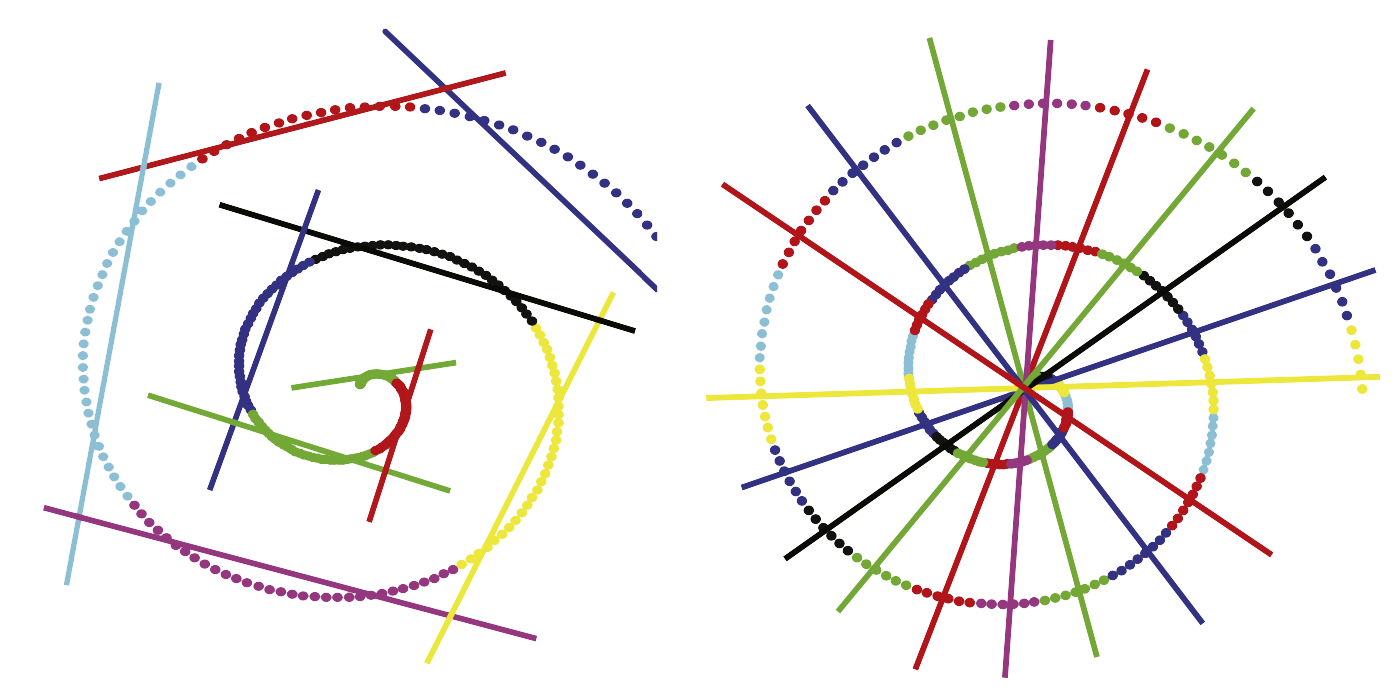
\includegraphics[width=0.7\textwidth]{goodandbadapprox.eps}
\caption{A sinistra una buona approssimazione di una varieta' 1D immersa in $\RR^{2}$ dove i colori rappresentano i diversi gruppi di punti approssimati da linee. A destra una cattiva approssimazione che non preserva la geometria della varieta'.}
\end{figure}
\es

\bs
\bc{\bf\color{blue}Framework}\ec
\begin{definition}[Varieta']
Un insieme $M\subseteq\RR^{N}$ e' detto varieta' differenziabile di dimensione $d$ se $\forall x\in M$ esiste un aperto $V\subseteq\RR^{N}$ t.c. $x\in V$ e un aperto $W\subseteq\RR^d$ ed esiste $f:W\to\RR^{N}$ iniettiva, differenziabile e ad inversa continua t.c.
\begin{itemize}
  \item $f(W)=M\cap V$ e
  \item $Rank(Df(y)) = d\ \forall y\in W$ (Dove $Df$ indica la Jacobiana di $f$)
\end{itemize}
\end{definition}
Supponiamo $f(a)=x$ allora la matrice $Df(a)$ e la corrispondente trasformazione lineare $f_{*}:\RR^{d}_{a}\to \RR^{N}_{x}$ definiscono un sottospazio di dimensione $d$ detto lo spazio tangente a $M$ in $x$ denotato $M_{x}$. \\
Per comodita' indicheremo da qui in poi con $M_x$ lo spazio tangente ad $M$ in $x$ traslato pero' all'origine di $\RR^N$.

\begin{figure}[b]
\centering
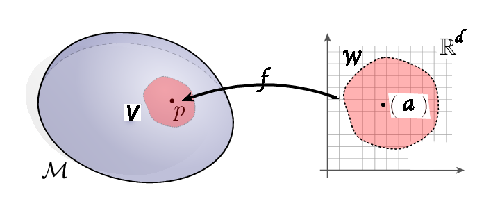
\includegraphics[width=0.5\textwidth]{manifold.eps}
\end{figure}
\es

\bs
\bc{\bf\color{blue}Osservazione motivante}\ec
E' fondamentale osservare che se per opportuni $x, V$ e $W \ f$ e' lineare allora $Df(a)=Df(b) \ \forall a, b\in W$ e dunque lo spazio tangente di tutti i punti in $M\cap V$ coincide (a meno di una traslazione) e la regione di spazio puo' essere perfettamente rappresentata con dei sottospazi affini.
Siamo allora interessati a determinare regioni dove la $\it{variazione}$ dello spazio tangente nei diversi punti e' bassa (cosi' $Df(a)\approx Df(b)$). \\
Definiamo dunque una metrica tra spazi tangenti.
\es

\bs
\bc{\bf\color{blue}Grassmann Manifold e Geodetiche}\ec
L'insieme dei sottospazi lineari di dimensione $d$ di $\RR^{N}$ e' detto Grassmanniana indicato $G_{N,d}(\RR^{N})$. In $G_{N,d}(\RR^{N})$ e' definita la distanza geodetica tra due sottospazi a partire dai loro angoli principali. In particolare possiamo definire la distanza tra $M_x$ e $M_y$ come

\begin{wrapfigure}{r}{0.4\textwidth}
    \centering
    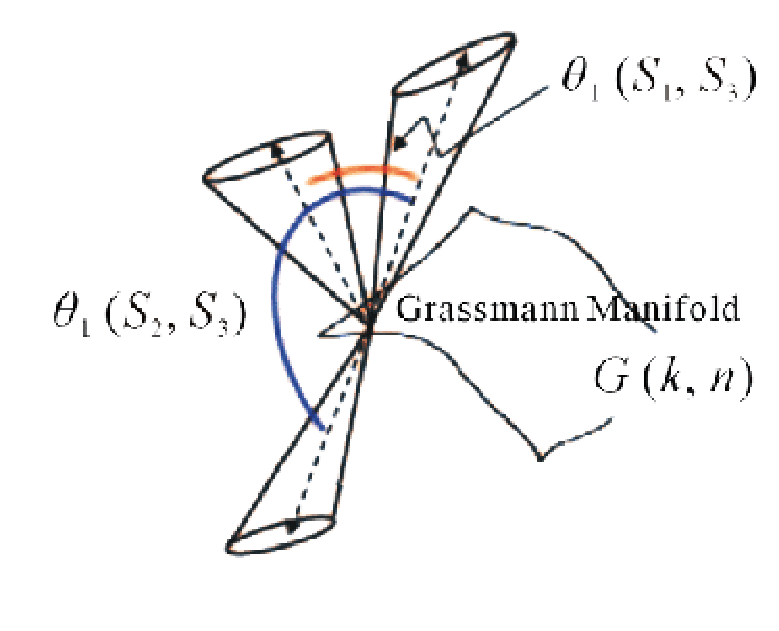
\includegraphics[width=0.4\textwidth]{principalangles.eps}
\end{wrapfigure}

\begin{equation*}
	D_{T}\left(M_{x}, M_{y}\right)=\left(\sum_{i=1}^{d} \theta_{i}^{2}\right)^{2}=\|\theta\|_{2}
\end{equation*}

dove $\theta=\left\{\theta_{1}, \ldots, \theta_{d}\right\}$ e' il vettore \\ degli angoli principali di $M_x$ e $M_y$. 
\es

\bs
\bc{\bf\color{blue}Punto medio di Karcher}\ec
Siamo inoltre interessati a poter calcolare una generalizzazione della media aritmetica applicata alla Grassmanniana.
\begin{definition}[Punto medio di Karcher su $G_{N,d}(\RR^{N})$ con distanza geodetica]
Il punto medio di un insieme $C$ di punti di $G_{N,d}(\RR^{N})$ rispetto alla distanza $D_T$ e' dato da
\begin{equation*}
M_{C}=\underset{M \in G_{N, d}}{\arg \min } \sum_{x \in C} D_{T}^{2}\left(M_{x}, M_{C_{i}}\right)
\end{equation*}
\end{definition}
Esistono vari metodi per risolvere in $M_C$ la precedente equazione, qui viene usata una formulazione data da $\it{J.M. Chang}$ che sfrutta la decomposizione in valori singolari (SVD).
\es

\bs
\bc{\bf\color{blue}Clustering}\ec
Sia $\mathcal{X} = \{x_k\in\RR^N, k\in [1, m]\}$ la rappresentazione di una varieta' attraverso un insieme di suoi punti. Sia $G_{\mathcal{X}}=G(\mathcal{X}, E)$ il grafo simmetrico non orientato che rappresenta la geometria della varieta'. Vogliamo determinare $\textbf{C}_{\mathcal{L}}=\{C_i, i\in [1, \mathcal{L}]\}$ partizione di $\mathcal{X}$ tale che $\forall i\ C_i$ possa essere ben rappresentato da un sottospazio affine che rispetti la geometria della varieta'.
\begin{definition}[Partizione]
$\textbf{C}_{\mathcal{L}}$ e' una partizione se $C_i\cap C_j = \emptyset \ \forall i\neq j, \ i,j\in \{1, ..., \mathcal{L} \}$ e $\bigcup_{i} C_i = \mathcal{X}$.
\end{definition}
Non tutte le partizione saranno pero' valide una condizione sufficiente e' che la partizione sia formata solo da cluster con sottografi connessi.
\begin{definition}[Sottografo connesso]
Dato $G_{C_i}=G(C_i, E_i)$ sottografo dove $E_i=\{a_{ij}\in E: \ x_i, x_j\in C_i\}$ diciamo che esso e' connesso se ogni coppia di nodi $x_i, x_j\in C_i$ e' connessa.
\end{definition}
\es

\bs
\bc{\bf\color{blue}Validita'}\ec
Denotiamo l'insieme delle partizioni valide $\Phi_\mathcal{L}(\mathcal{X})$.
\begin{definition}[Predicato di $\it{validita'}$]
$\Phi_\mathcal{X}(\textbf{C}_\mathcal{L}) \equiv \textbf{C}_\mathcal{L}\in \Phi_\mathcal{L}(\mathcal{X})$ definito come
\begin{equation*}
\begin{gathered}
\Phi_\mathcal{X}(\textbf{C}_\mathcal{L}) = \bigwedge_{C_i\in\textbf{C}_\mathcal{L}}\phi(C_i) \\
\phi(C_i) = 
  \begin{cases}
                                   Vero & \text{Se $C_i$ e' connesso} \\
                                   Falso & \text{altrimenti} \\
  \end{cases}
\end{gathered}
\end{equation*}
\end{definition}
\bc{\bf\color{blue}Fondibilita'}\ec
Possiamo definire anche un predicato di fondibilita' $\Psi$ che descrive se due cluster possono essere uniti dando vita a una partizione ancora valida, i predicati di fondibilita' e validita' sono legati dalla relazione seguente: \\
Se $C_i,C_j\neq \emptyset, C_i\cap C_j =\emptyset, \ \phi(C_i)\wedge\phi(C_j)$ e $\Psi(C_i, C_j) \implies \phi(C_i\cup C_j)$
Evitando una definizione formale, due cluster saranno fondibili se esiste un $\it{edge}$ che li collega.
\es

\bs
\begin{figure}[t]
\centering
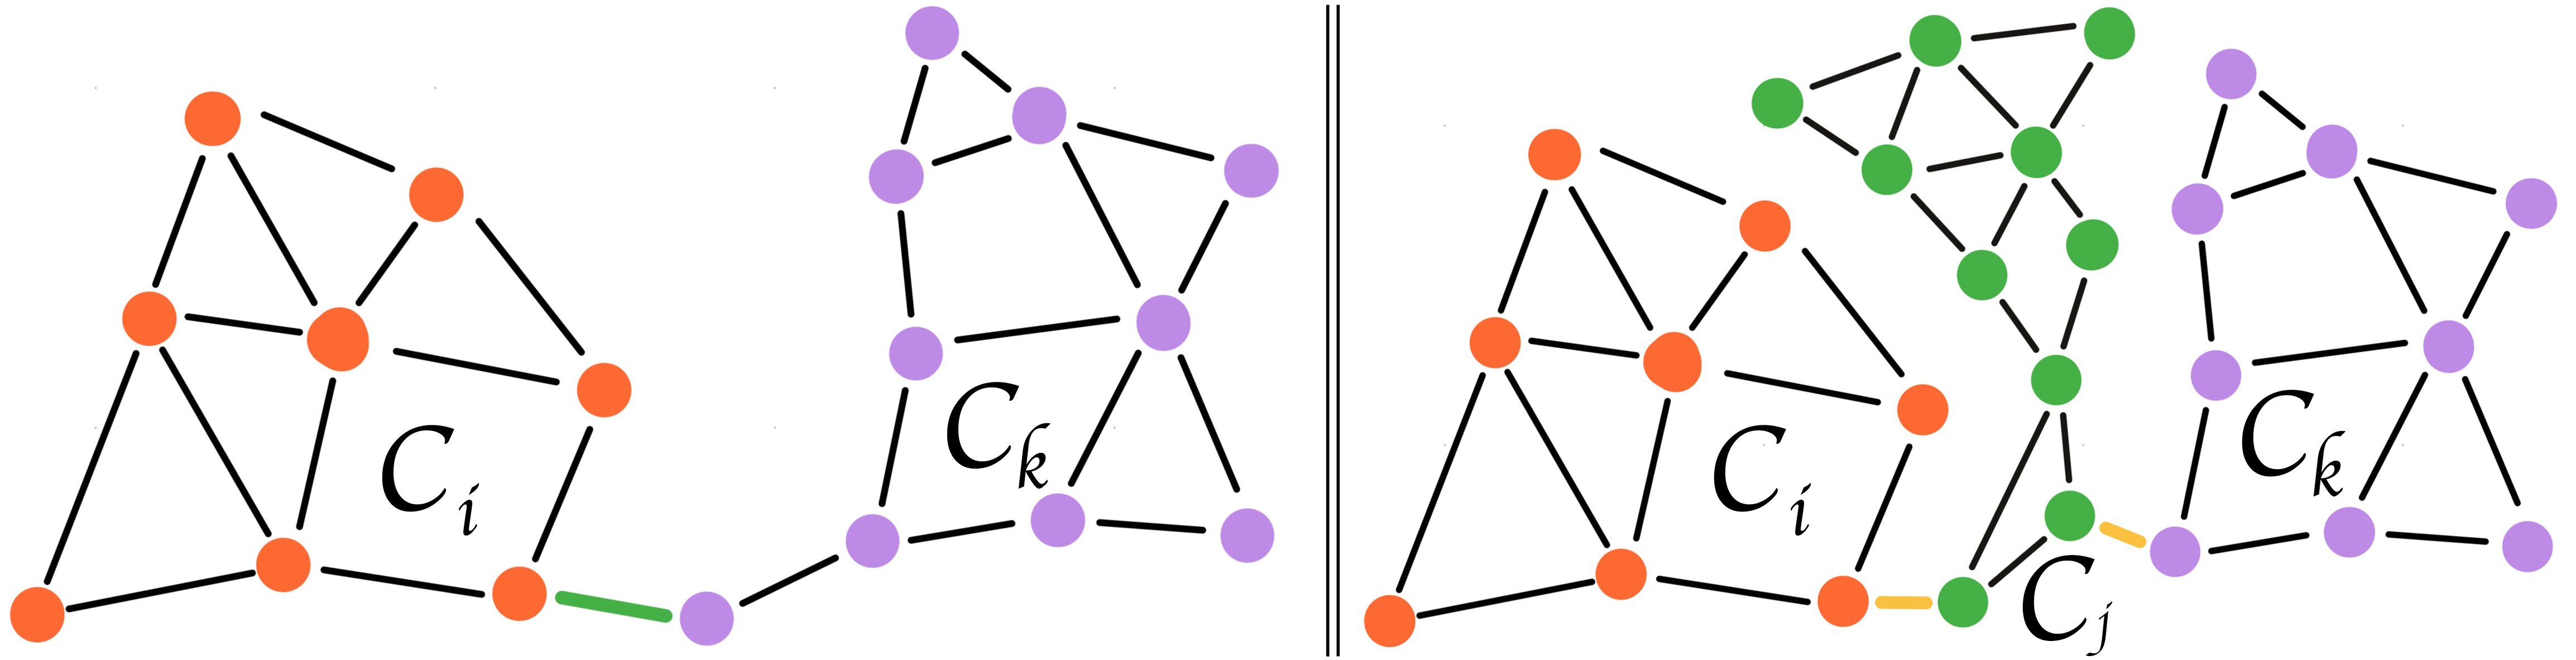
\includegraphics[width=1\textwidth]{connectedclusters.eps}
\caption{A sinistra due cluster $C_i$ e $C_k$ connessi e dunque fondibili. A destra tre cluster dove sia $C_i$ che $C_k$ sono fondibili con $C_j$ ma $C_i$ e $C_k$ non sono fondibili. \\
E' facile osservare che fondendo le coppie (fondibili) in entrambe le configurazioni la partizione risultante e' composta da sottografi connessi e dunque valida.}
\end{figure}
\es

\bs
\bc{\bf\color{blue}Bonta' di una partizione}\ec
Cerchiamo ora una funzione $\mathcal{P}$ che valuti la bonta' di una partizione, definiamo
\begin{equation*}
\begin{gathered}
	\mathcal{P}(\textbf{C}) = \sum_{C_i\in\textbf{C}}p(C_i) \ \ \text{con} \\
	p(C_i) = \sum_{x\in C_i}D^{2}_T(M_{C_i}, M_x)
\end{gathered}
\end{equation*}
Osserviamo che per definizione $\mathcal{P}$ e' distributiva sui cluster e non negativa, inoltre e' nulla sui cluster formati da singoletti.

\bc{\bf\color{blue}Il problema di approssimazione}\ec
Ora che abbiamo una misura di bonta' possiamo definire il nostro problema di approssimazione come la ricerca della partizione $\mathbf{C}_{\mathcal{L}}^{*}(\mathcal{X})$ dove
\begin{equation*}
\mathbf{C}_{\mathcal{L}}^{*}(\mathcal{X})=\underset{\mathbf{C} \in \Phi_{\mathcal{L}}(\mathcal{X})}{\operatorname{argmin}} \mathcal{P}(C)= \underset{\mathbf{C} \in \Phi_{\mathcal{L}}(\mathcal{X})}{\operatorname{argmin}} \sum_{C_{i} \in \mathbf{C}} \sum_{x \in C_{i}} D_{T}^{2}\left(M_{C_{i}}, M_{x}\right)
\end{equation*}
\es

\bs
\bc{\bf\color{blue}Verso una formulazione greedy}\ec
Vogliamo formulare una versione meno accurata ma piu' efficiente,
introduciamo alcuni rilassamenti al problema andando a determinare un algoritmo greedy e bottom-up, ci serve pero' un modo per valutare la bonta' di una fusione di cluster.
\begin{definition}[Misura di Dissimilarita']
$d:(C_i, C_j)\to R^{+}_0$ \\
$d(C_i, C_j) = p(C_i\cup C_j) - p(C_i) - p(C_j)$ \\
\end{definition}
Esplicitando possiamo osservare che $d\geq 0$ infatti
\es

\bs
\begin{equation*}
\begin{aligned}
d\left(C_{i}, C_{j}\right)=& \sum_{x \in C_{i} \cup C_{j}} D_{T}^{2}\left(M_{x}, M_{C_{i} \cup C_{j}}\right)-\sum_{x \in C_{i}} D_{T}^{2}\left(M_{x}, M_{C_{i}}\right) \\
&-\sum_{x \in C_{j}} D_{T}^{2}\left(M_{x}, M_{C_{j}}\right) \\
=& \sum_{x \in C_{i}} \left[D_{T}^{2}\left(M_{x}, M_{C_{i} \cup C_{j}}\right)- D_{T}^{2}\left(M_{x}, M_{C_{i}}\right)\right] \\
&+\sum_{x \in C_{j}} \left[D_{T}^{2}\left(M_{x}, M_{C_{i} \cup C_{j}}\right)-D_{T}^{2}\left(M_{x}, M_{C_{j}}\right)\right]
\end{aligned}
\end{equation*}
Da cui segue la tesi data la definizione di $M_{C_i}$, $M_{C_j}$ e $M_{C_i\cup C_j}$. \\
Possiamo allora riscrivere il nostro problema nella forma
\vskip 0.05in
$\mathbf{C}_{\mathcal{L}}^{*}(\mathcal{X})=\left(\mathbf{C}_{\mathcal{L}+1}^{\prime}(\mathcal{X}) \backslash\left\{C_{i}^{\prime}, C_{j}^{\prime}\right\}\right) \cup\left\{C_{i}^{\prime} \cup C_{j}^{\prime}\right\}$ \ dove \\
$\left(\mathbf{C}_{\mathcal{L}+1}^\prime(\mathcal{X}), C_{i}^{\prime}, C_{j}^{\prime}\right)=\underset{C_{i}, C_{j} \in \mathbf{C}, \ \mathbf{C} \in \Phi_{\mathcal{L}+1} \atop \Psi(C_i, C_j) \ \text{e' vera}}{\operatorname{argmin}}\left(P(\mathbf{C})+d(C_{i}, C_{j})\right)$
\es

\bs
\bc{\bf\color{blue}Approccio dinamico e greedy relaxation}\ec
Questa formulazione permette un approccio dinamico, per avere la migliore partizione di $\mathcal{L}$ cluster possiamo controllare tutte le partizioni di $\mathcal{L} + 1$ cluster e unire i due cluster a minor costo. \\
Deriviamo un algoritmo greedy togliendo la ricerca su $\Phi_{\mathcal{L}+1}$ e otteniamo
\vskip 0.05in
$\widehat{\mathbf{C}}_{\mathcal{L}}(\mathcal{X})=\left(\mathbf{C}_{\mathcal{L}+1}(\mathcal{X}) \backslash\left\{C_{i}^{\prime}, C_{j}^{\prime}\right\}\right) \cup\left\{C_{i}^{\prime} \cup C_{j}^{\prime}\right\}$ \\
dove \ $\left(C_{i}^{\prime}, C_{j}^{\prime}\right)=\underset{C_{i}, C_{j} \in \widehat{\mathbf{C}}_{\mathcal{L} + 1}(\mathcal{X}) \atop \Psi(C_i, C_j) \ \text{e' vera}}{\operatorname{argmin}}d(C_{i}, C_{j})$ \\
Questo riduce notevolmente il costo computazionale ma non assicura piu' l'ottimalita' della soluzione trovata. \\
\vskip 0.1in
Siamo ora pronti a descrivere l'algoritmo di clustering.
\es

\bs
\bc{\bf\color{blue}Inizializzazione: $G_\mathcal{X}$ e $M_x$}\ec
$G_\mathcal{X}$ e' costruita connettendo ogni punto ai suoi vicini attraverso una $\it{knn}$, per ogni punto $x\in\mathcal{X}$
definiamo inoltre $N_x = \{y\in\mathcal{X} : \left( x, y \right) \in E \}$ l'insieme dei neighbors di $x$.
Ora $M_x$ puo' essere approssimato come il sottospazio di dimensione $d$ che meglio approssima $N^{0}_x$. \\
Per il teorema di $\it{Eckart}$\ -$\it{Young}$ questo corrisponde a determinare la $d$-$rank$ SVD di $\left[N^{0}_x\right]$.
\bc{\bf\color{blue}Algoritmo di merging}\ec
Fissiamo $n=|\mathcal{X}|$ e la partizione iniziale ottimale $C^{*}_n = \{\{x\}; x\in\mathcal{X}\}$ \\
Ad ogni iterazione uniamo due cluster $C_i$ e $C_j$, Il predicato di fondibilita' precedentemente definito ci permette
di determinare tutti i possibili $C_i$ e $C_j$ fondibili: essi saranno i cluster che sono connessi per almeno un $\it{edge}$.
La dissimilarita' tra due cluster era definita come
\begin{equation*}
\begin{aligned}
d(C_i, C_j) =& \ p(C_i\cup C_j) - p(C_i) - p(C_j) \\
=& \sum_{x \in C_{i}} \left[D_{T}^{2}\left(M_{x}, M_{C_{i} \cup C_{j}}\right)- D_{T}^{2}\left(M_{x}, M_{C_{i}}\right)\right] \\
&+\sum_{x \in C_{j}} \left[D_{T}^{2}\left(M_{x}, M_{C_{i} \cup C_{j}}\right)-D_{T}^{2}\left(M_{x}, M_{C_{j}}\right)\right]
\end{aligned}
\end{equation*}
\es

\bs
Tale equazione e' costosa da computare poiche' richiede il calcolo di $M_{C_i\cup C_j}$ per ogni ipotetica fusione.
Vorremmo una formulazione che dipenda solo da valori gia' calcolati e.g. lo spazio tangente medio di ogni cluster e
la distanza tra esso e gli spazi tangenti dei singoli punti del cluster. \\
Osserviamo $\sum_{x \in C_{i}} D_{T}^{2}\left(M_{x}, M_{C_{i} \cup C_{j}}\right) \leq \sum_{x \in C_{i}} D_{T}^{2}\left(M_{x}, M_{C_{j}}\right)$, provabile p.a.
Lo stesso vale naturalmente per $C_j$, allora sostituendo in $d$ otteniamo:
\begin{equation*}
\begin{aligned}
  d\left(C_{i}, C_{j}\right) \leq & \sum_{x \in C_{i}}\left[\textcolor{red}{D_{T}^{2}\left(M_{x}, M_{C_{j}}\right)}-D_{T}^{2}\left(M_{x}, M_{C_{i}}\right)\right] \\
  &+\sum_{x \in C_{j}}\left[\textcolor{red}{D_{T}^{2}\left(M_{x}, M_{C_{i}}\right)}-D_{T}^{2}\left(M_{x}, M_{C_{j}}\right)\right]
  \end{aligned}
\end{equation*}
Ora per la disuguaglianza triangolare si ha
\begin{equation*}
  \begin{array}{ll}
    \textcolor{red}{D_{T}\left(M_{x}, M_{C_{j}}\right)} \leq D_{T}\left(M_{x}, M_{C_{i}}\right)+D_{T}\left(M_{C_{i}}, M_{C_{j}}\right), & \forall x \in \mathcal{X} \\
    \textcolor{red}{D_{T}\left(M_{x}, M_{C_{i}}\right)} \leq D_{T}\left(M_{x}, M_{C_{j}}\right)+D_{T}\left(M_{C_{i}}, M_{C_{j}}\right), & \forall x \in \mathcal{X}
    \end{array}
\end{equation*}
\es

\bs
E quindi elevando al quadrato e sommando sui punti di $C_i$ e $C_j$ rispettivamente otteniamo
\begin{equation*}
\begin{aligned}
  &\sum_{x \in C_{i}}\left[\textcolor{red}{D_{T}^{2}\left(M_{x}, M_{C_{j}}\right)}-D_{T}^{2}\left(M_{x}, M_{C_{i}}\right)\right] \\
  &\quad \leq 2 D_{T}\left(M_{C_{i}}, M_{C_{j}}\right) \sum_{x \in C_{i}} D_{T}\left(M_{x}, M_{C_{i}}\right)+\left|C_{i}\right| D_{T}^{2}\left(M_{C_{i}}, M_{C_{j}}\right) \\
  &\sum_{x \in C_{j}}\left[\textcolor{red}{D_{T}^{2}\left(M_{x}, M_{C_{i}}\right)}-D_{T}^{2}\left(M_{x}, M_{C_{j}}\right)\right] \\
  &\quad \leq 2 D_{T}\left(M_{C_{i}}, M_{C_{j}}\right) \sum_{x \in C_{j}} D_{T}\left(M_{x}, M_{C_{j}}\right)+\left|C_{j}\right| D_{T}^{2}\left(M_{C_{i}}, M_{C_{j}}\right)
  \end{aligned}
\end{equation*}
Otteniamo cosi' la formula finale per la nostra dissimilarita' approssimata $\tilde{d}$ che dipende \underline{solo}
da informazioni pregresse
\begin{equation*}
  \begin{aligned}
    &d\left(C_{i}, C_{j}\right) \leq\left(\left|C_{i}\right|+\left|C_{j}\right|\right) D_{T}^{2}\left(M_{C_{i}}, M_{C_{j}}\right) \\
    &\quad+2 D_{T}\left(M_{C_{i}}, M_{C_{j}}\right)\left[\sum_{x \in C_{i}} D_{T}\left(M_{x}, M_{C_{i}}\right)+\sum_{x \in C_{j}} D_{T}\left(M_{x}, M_{C_{j}}\right)\right]
  \end{aligned}
\end{equation*}
Calcoleremo cosi' lo spazio tangente medio solo per il nuovo cluster creato.
\es

\bs
\bc{\bf\color{blue}Schema dell'algoritmo completo}\ec
\begin{figure}[b]
\centering
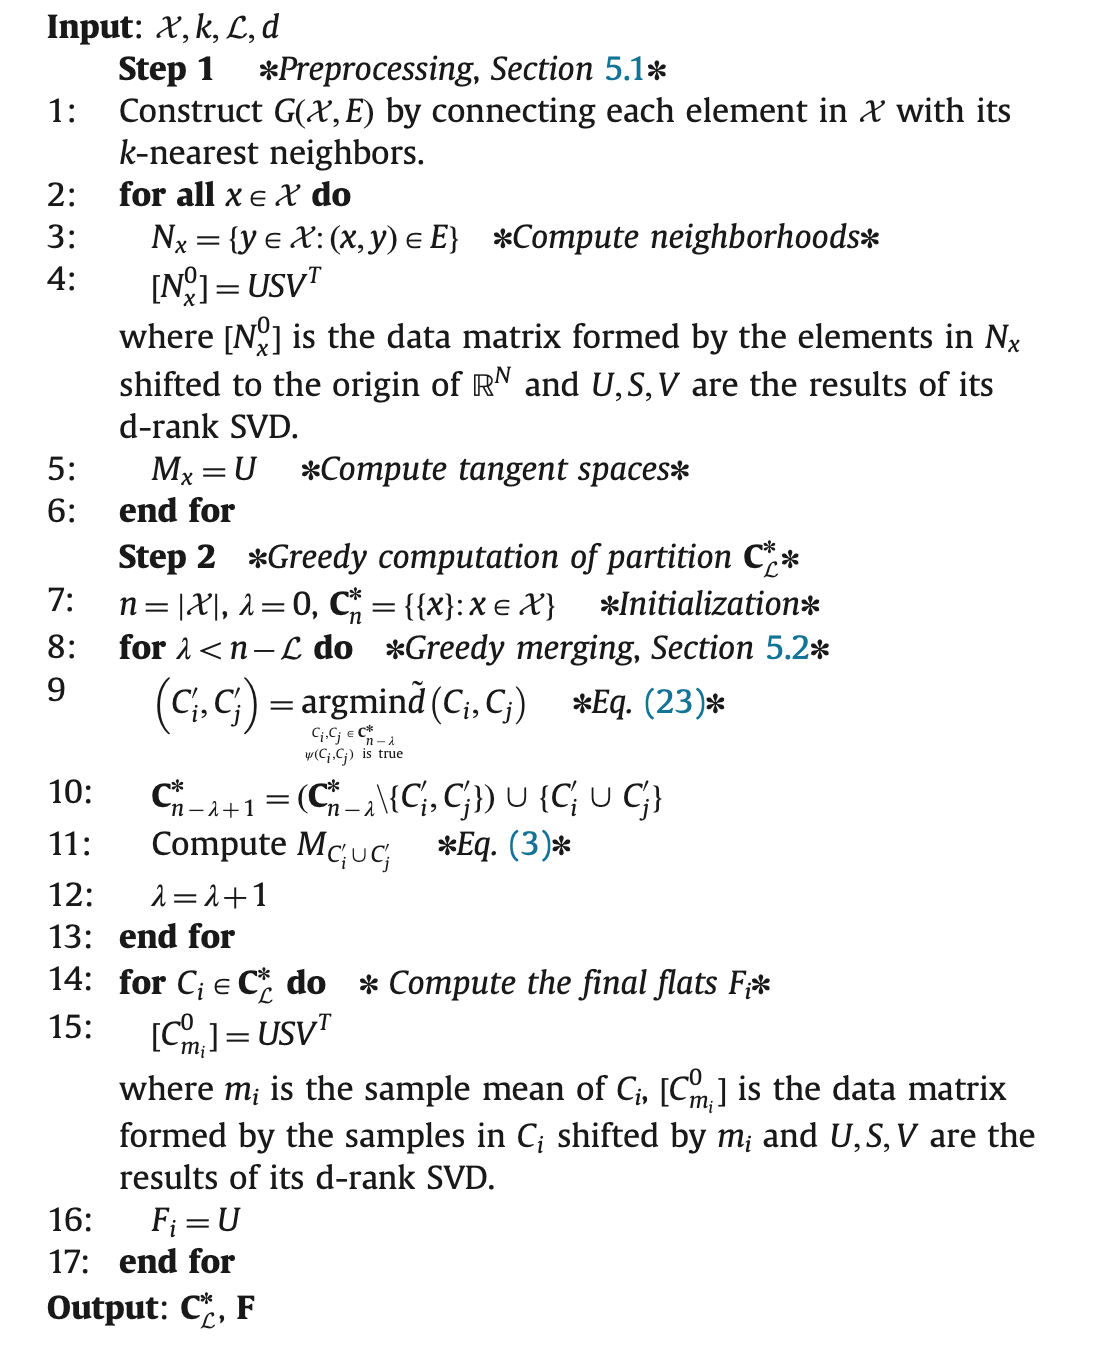
\includegraphics[width=0.55\textwidth]{algorithm.eps}
\end{figure}
Nelle linee $14-16$ vengono computati i sottospazi affini finali attraverso SVD.
\es

\bs
\bc{\bf\color{blue}Risultati sperimentali}\ec
Iniziamo con l'approssimazione di 2 dataset sintetici 3D, la Swiss Roll e la S-Curve. I test sono condotti con 5000 punti,
un neighborhood size di $k=15$ e $d=2$, la performance e' valutata con il $\it{mean\ squared\ reconstruction\ error.}$
$M S R E=\frac{1}{N} \sum_{i=1}^{N}\left\|x_{i}-\hat{x}_{i}\right\|^{2}$. \\
Riportiamo anche i tempi di esecuzione dell'algoritmo su tali dataset:
\begin{center}
    \begin{tabular}{ |c|c|c|c| }
    \hline
    Paper - MBP 2.66Ghz & Mine - MBA 1.6Ghz & Mine - i5 3.60GHz \\
    389s & \color[HTML]{009901} 267s & \color[HTML]{009901} 123s \\
    \hline
    \end{tabular}
\end{center}
\es

\bs
\bc{\bf\color{blue}Cluster finali S-Curve}\ec
\begin{figure}[b]
\centering
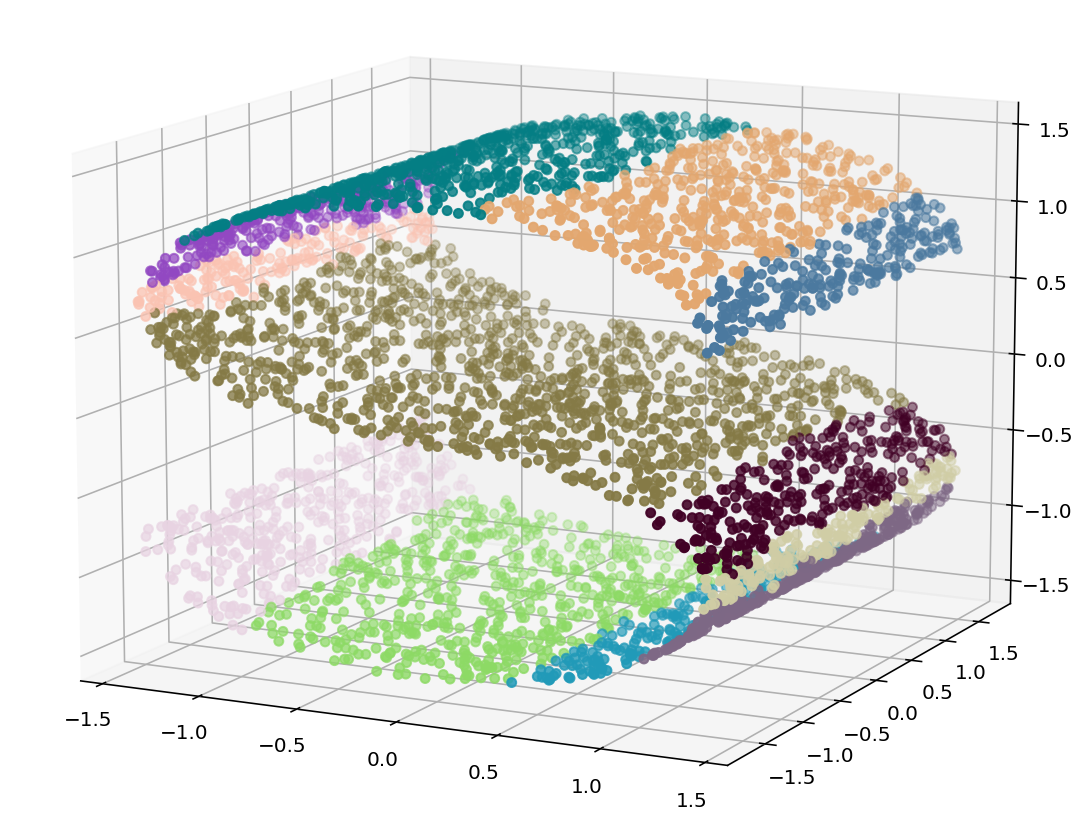
\includegraphics[width=0.95\textwidth]{scurve.eps}
\end{figure}
\es

\bs
\bc{\bf\color{blue}Cluster finali Swiss Roll}\ec
\begin{figure}[b]
\centering
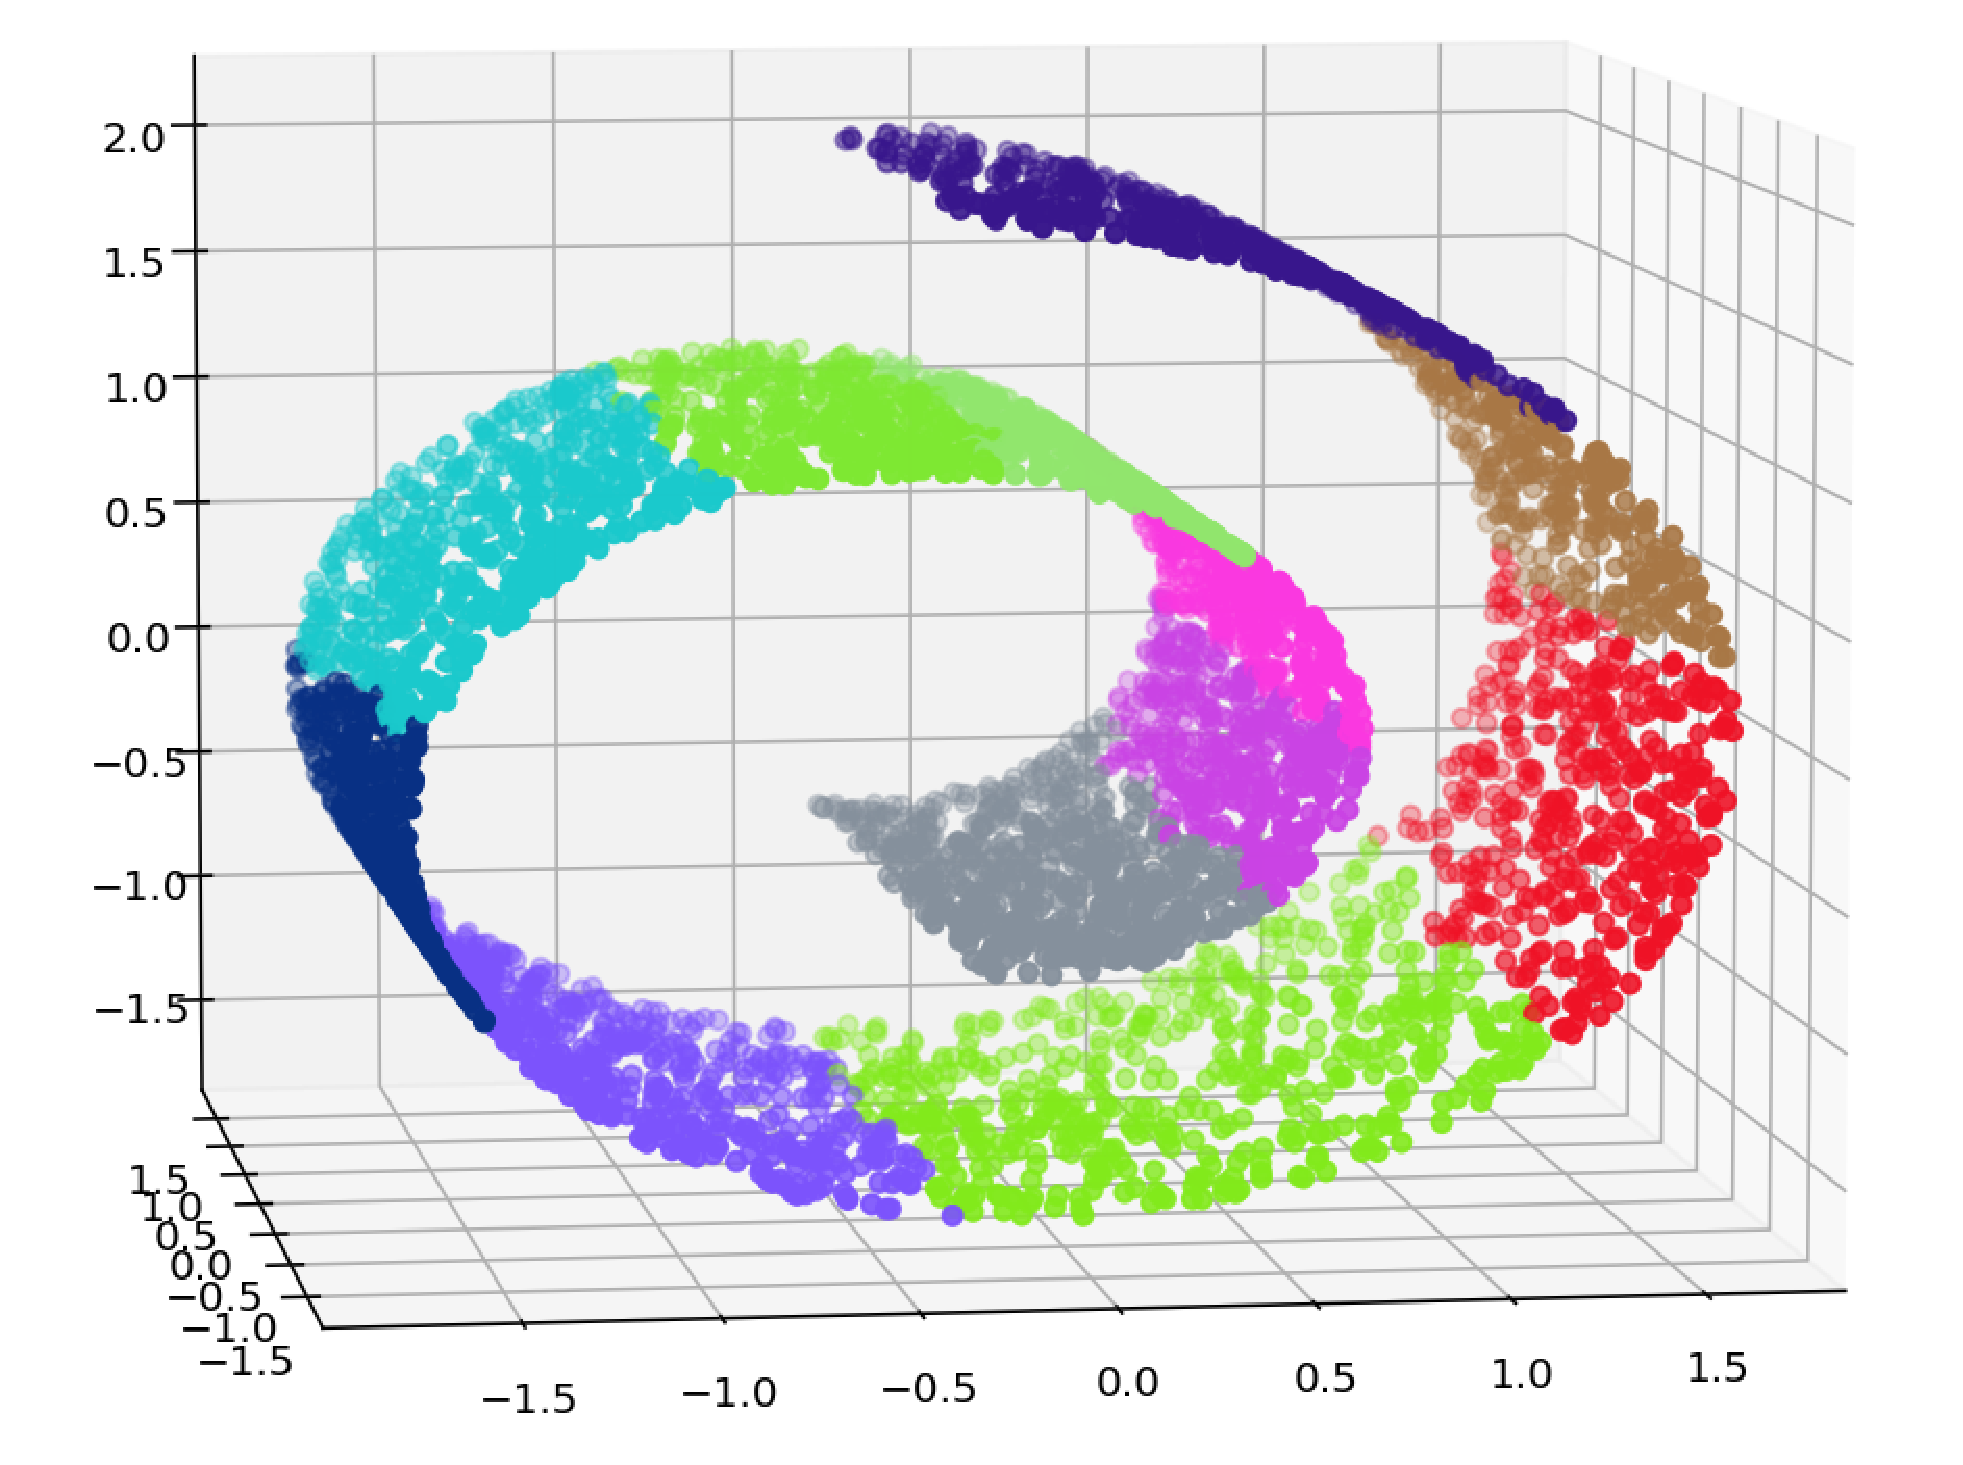
\includegraphics[width=0.95\textwidth]{swissroll.eps}
\end{figure}
\es

\bs
\begin{figure}[b]
\centering
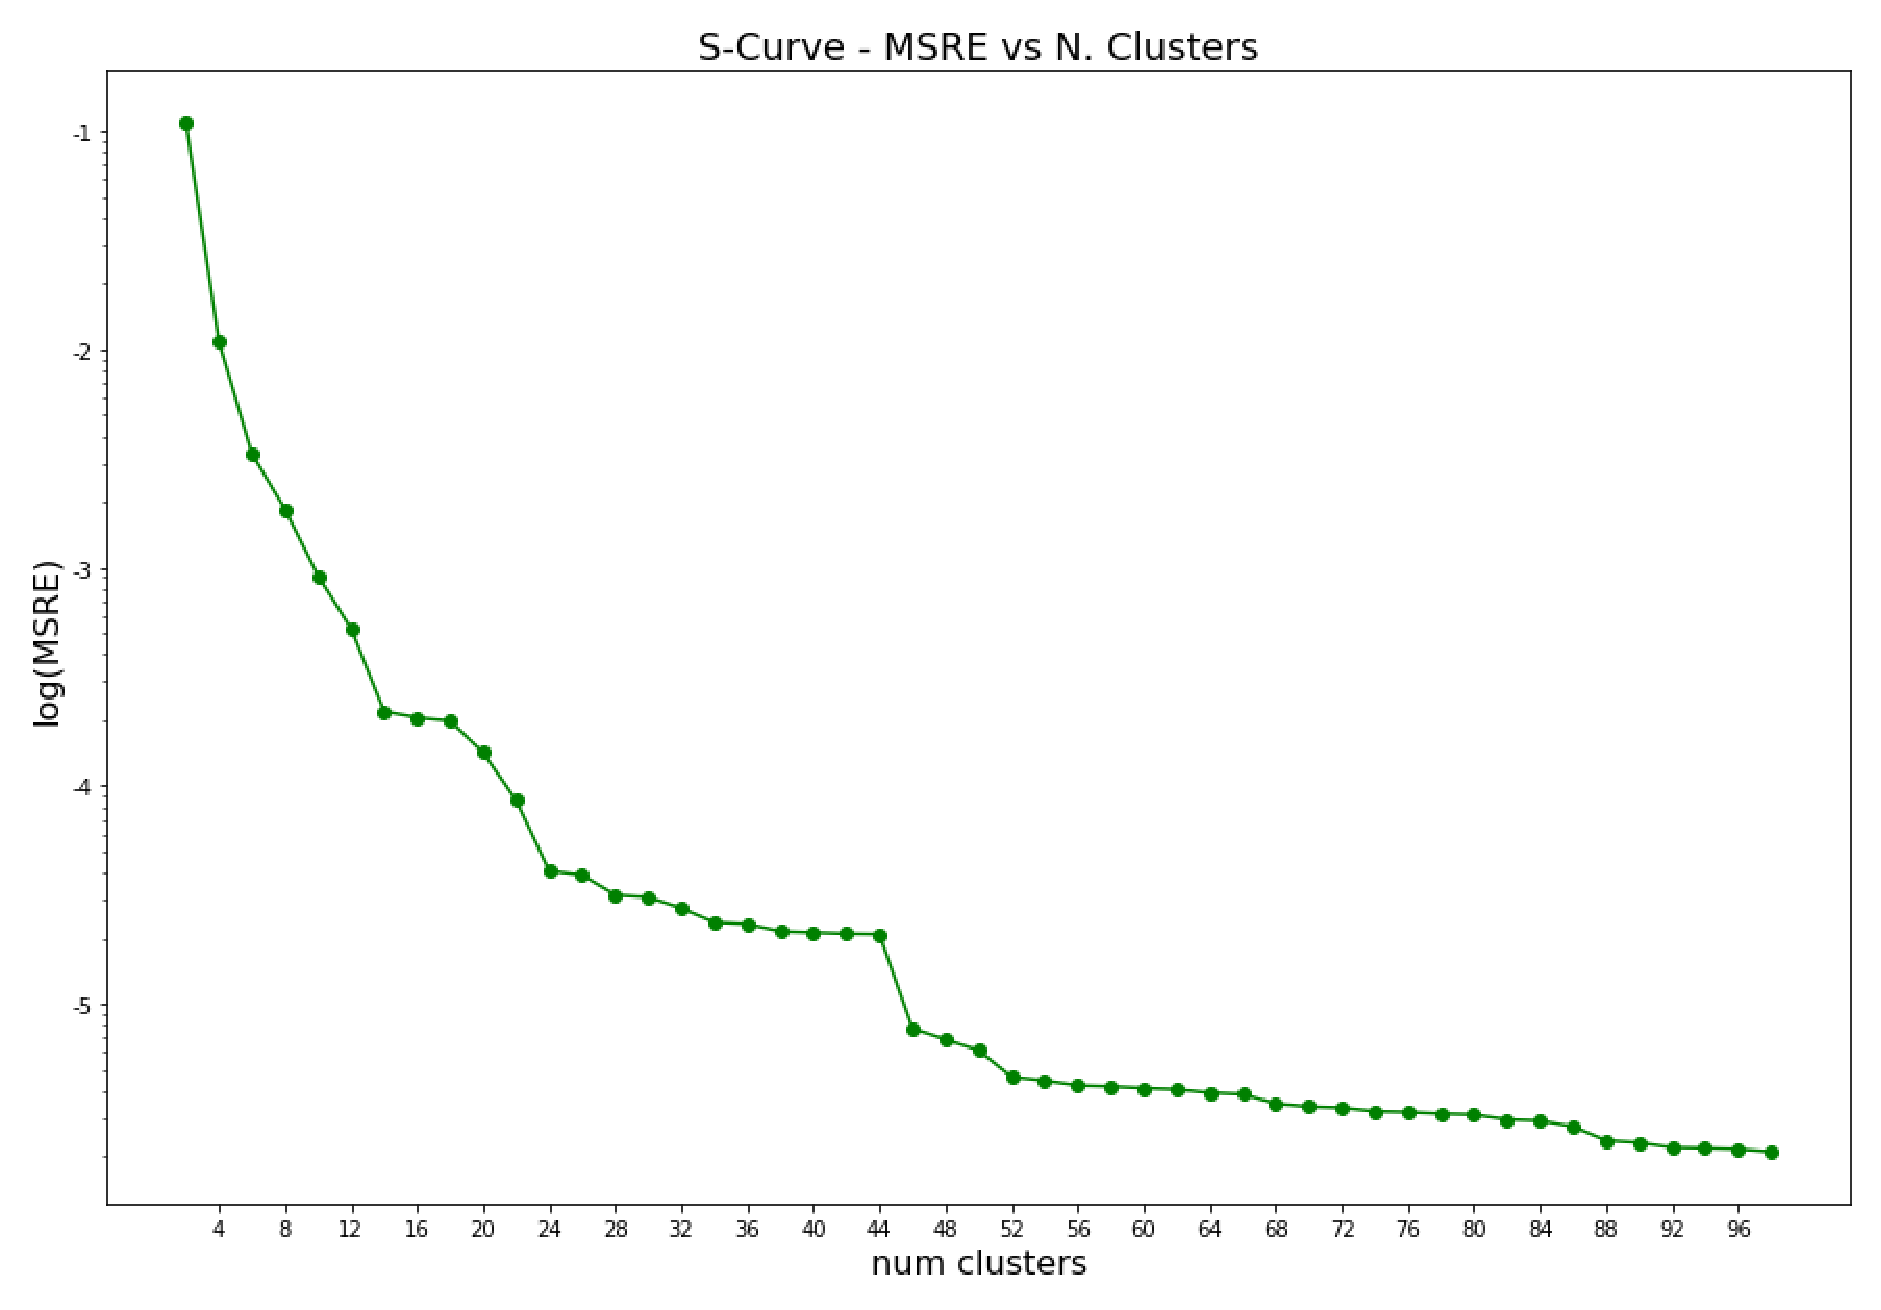
\includegraphics[width=\textwidth]{scurve_msre.eps}
\end{figure}
\es

\bs
\begin{figure}[b]
\centering
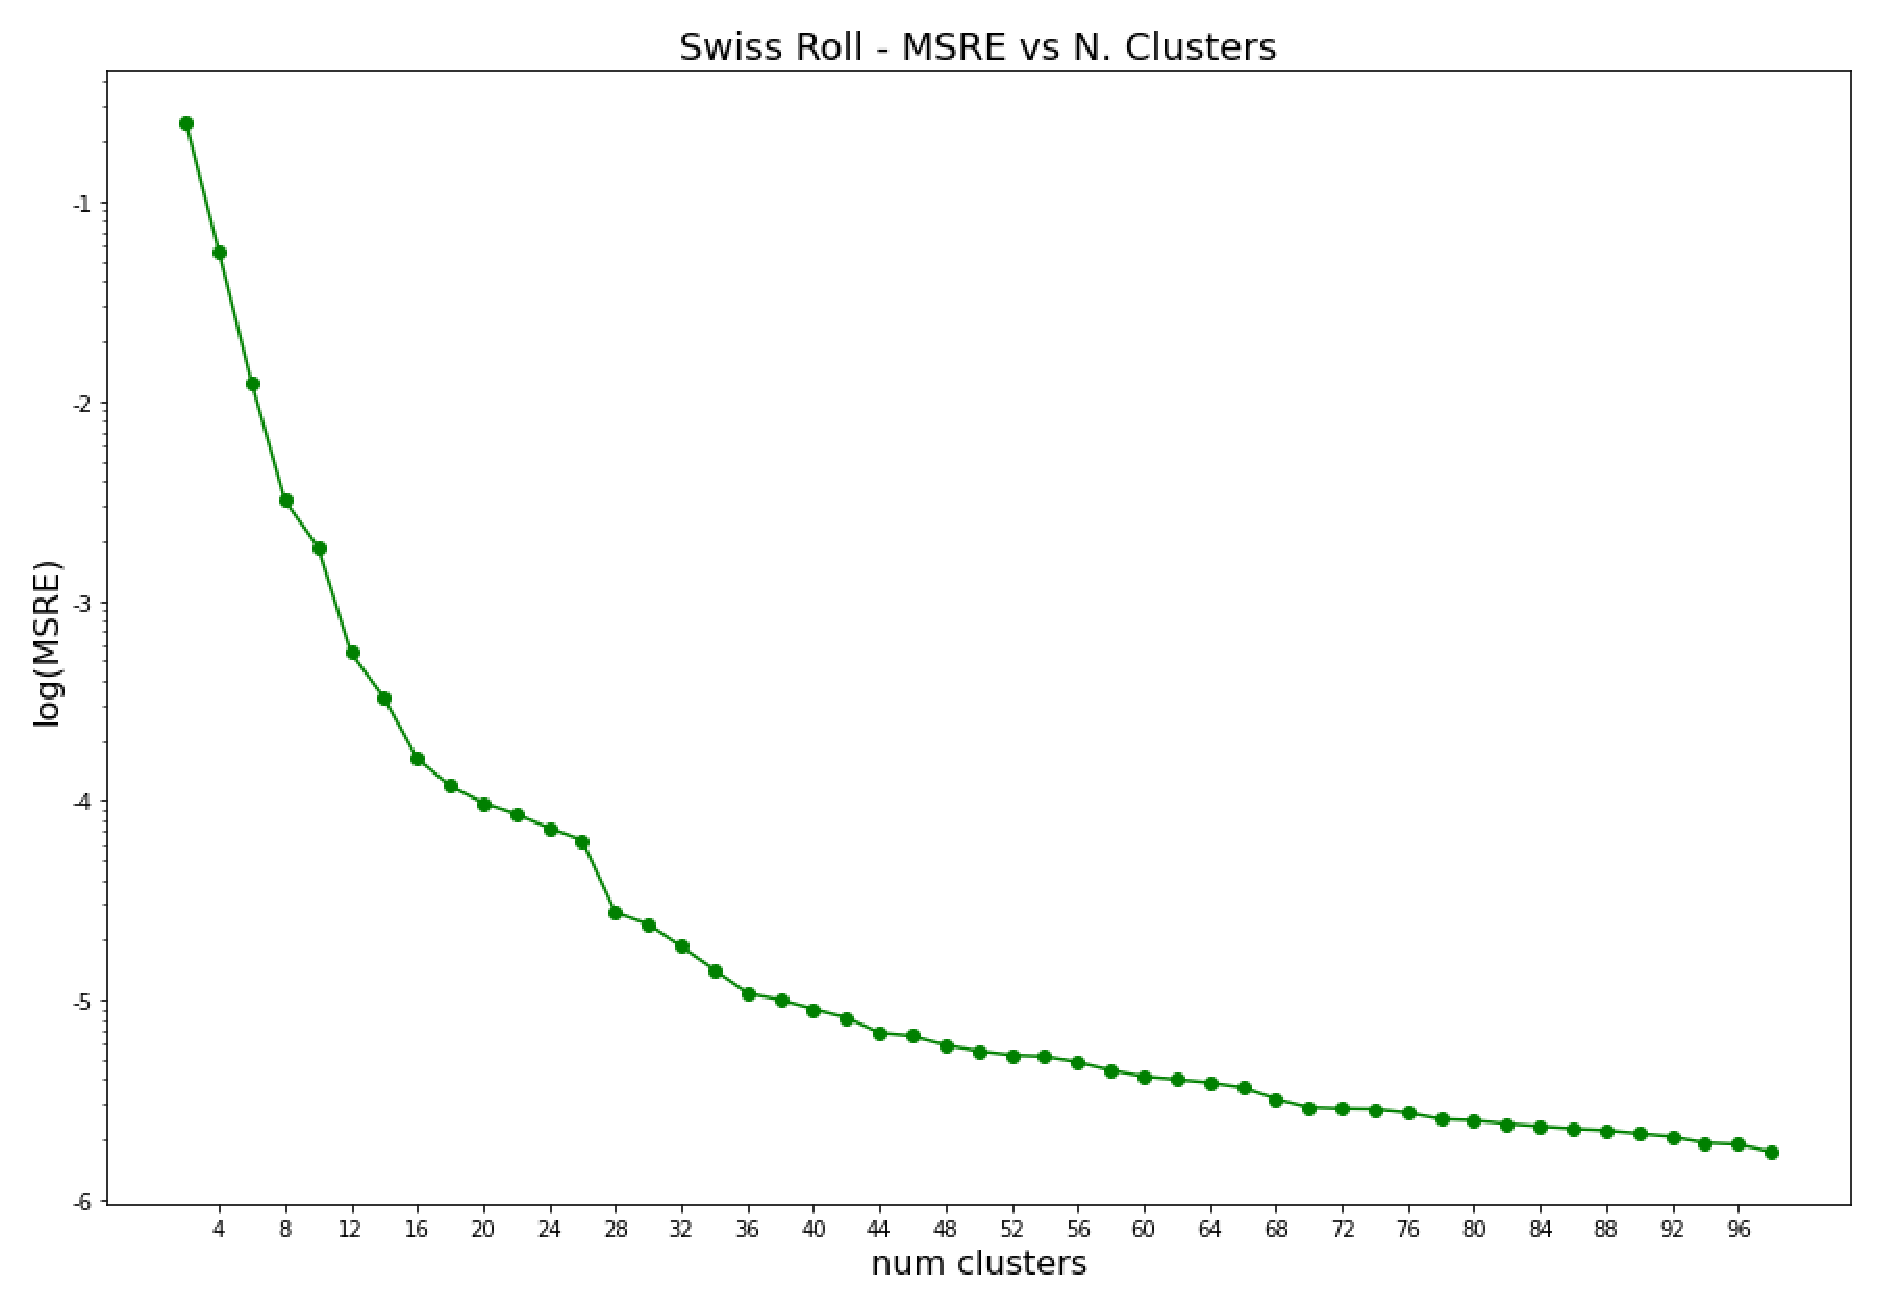
\includegraphics[width=\textwidth]{swiss_msre.eps}
\end{figure}
\es

\end{document}